\documentclass[12pt]{article}

\usepackage{amsmath}
\usepackage{unicode-math}
\usepackage{xltxtra}
\usepackage{xgreek}

\setmainfont{Liberation Serif}

\usepackage{tabularx}

\pagestyle{empty}

\usepackage{geometry}
 \geometry{a4paper, total={190mm,280mm}, left=10mm, top=10mm}

 \usepackage{graphicx}
 \graphicspath{ {images/} }

 \usepackage{wrapfig}

\begin{document}

\part*{\centering{Λύσεις}}

\section*{Θέμα Α}
  \noindent
  \begin{enumerate}
    \item Απόδειξη από σχολικό βιβλίο (το αντίστροφο δεν χρειάζεται).
    \item Από σχολικό βιβλίο... (αν είναι οι δύο κάθετες ίσες τότε Π-Γ-Π, αν είναι η υποτείνουσα και μία κάθετη τότε κριτήριο ορθογωνίων)
    \item Να χαρακτηρίσετε τις παρακάτω προτάσεις με Σωστό ή Λάθος
    \begin{enumerate}
      \item [α)] Λάθος
      \item [β)] Σωστό
      \item [γ)] Σωστό
      \item [δ)] Λάθος
      \item [ε)] Σωστό
    \end{enumerate}
  \end{enumerate}

\section*{Θέμα Β}
  \noindent
  \begin{enumerate}
    \item Κριτήριο Π-Γ-Π.
    \item Από το προηγούμενο ερώτημα.
    \item $ΑΔ$ διχοτόμος άρα και μεσοκάθετος.
  \end{enumerate}
  %\vspace{7\baselineskip}

\section*{Θέμα Γ}
  \noindent
  \begin{wrapfigure}{r}{0.5\textwidth}
    \centering
    \vspace{-60pt}
    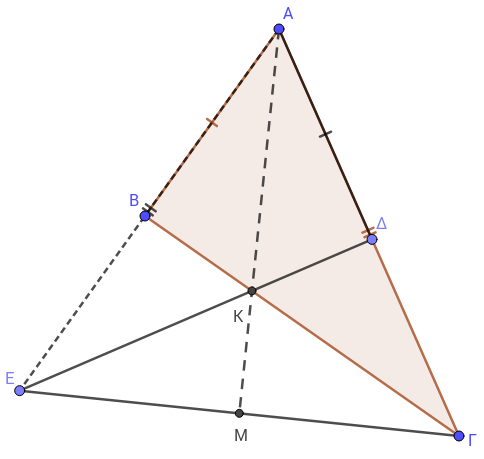
\includegraphics[width=0.5\textwidth]{2017AGeoDiagLyseis}
  \end{wrapfigure}
  \begin{enumerate}
    \item Π-Π-Π στα τρίγωνα $ΑΒΓ$ και $ΑΔΕ$
    \item Τα τρίγωνα $ΒΚΕ$ και $ΔΚΓ$ είναι ίσα (Γ-Π-Γ) αφού $ΕΚ=ΓΚ$ λόγω ότι $ΕΓΚ$ είναι ισοσκελές.
    \item Τα τρίγωνα $ΑΒΚ$ και $ΑΔΚ$ είναι ίσα (Π-Π-Π) άρα $ΑΚ$ διχοτόμος
    \item Διχοτόμος στο $ΑΕΓ$ που είναι ισοσκελές.
  \end{enumerate}

\vspace{3\baselineskip}

\end{document}
